\chapter{Como o som viaja}\label{ch:g4:how-sound-travels}

O clarão do relâmpago --- depois um, dois, três segundos de silêncio
--- e só agora o ronco do trovão. E olha que o clarão e o ronco
nasceram juntos, na mesma nuvem! O \omterm{def:g3:sound-around-us:sound}{som}, como aprendemos, é um tremor
que viaja. Este capítulo o acompanha na estrada: por onde ele viaja,
com que velocidade corre e o que acontece quando ele bate numa
parede.

\section{O som precisa de um transportador}

\begin{proposition}[Sem transportador, sem som]\label{prop:g4:how-sound-travels:carrier}
O \omterm{def:g3:sound-around-us:sound}{som} viaja apenas \emph{através} das coisas: pelo \omterm{def:g2:air-around-us:air}{ar}, pela água,
pela madeira, pelo tijolo e pelo aço. Onde não há absolutamente nada
--- nem \omterm{def:g2:air-around-us:air}{ar}, nem material de tipo nenhum --- o \omterm{def:g3:sound-around-us:sound}{som} não consegue
viajar: o tremor não tem o que fazer tremer.
\end{proposition}

\begin{example}[A campainha no frasco]\label{ex:g4:how-sound-travels:jar}
Uma experiência famosa, de três séculos atrás: uma campainha elétrica
toca dentro de um frasco de vidro --- e é ouvida com clareza. Uma
bomba então suga o \omterm{def:g2:air-around-us:air}{ar} do frasco lacrado enquanto o martelinho da
campainha continua batendo, bem visível. O toque vai sumindo\dots\ e
morre. Deixe o \omterm{def:g2:air-around-us:air}{ar} voltar correndo: o toque volta. A campainha nunca
parou --- foi o \emph{transportador} dela que foi tirado e devolvido.
E agora você pode resolver uma velha pergunta: a \omterm{def:g2:moon-in-the-sky:moon}{Lua} silenciosa, onde
um grito morre sem ser ouvido, é silenciosa porque não tem \omterm{def:g2:air-around-us:air}{ar} nenhum.
\end{example}

\begin{omfigure}
\begin{tikzpicture}[scale=0.85]
  \draw[thick] (0.7,0) -- (0.7,3.0) .. controls (0.7,3.5) and
    (3.3,3.5) .. (3.3,3.0) -- (3.3,0);
  \draw[thick] (0.2,0) -- (3.8,0);
  % the bell: hanger, dome with a flared skirt, mouth, clapper
  \draw[thick] (2.0,2.9) -- (2.0,2.45);
  \draw[thick, fill=yellow!65!orange]
    (1.42,1.52)
    .. controls (1.5,1.6) and (1.58,1.7) .. (1.6,1.85)
    .. controls (1.62,2.1) and (1.65,2.45) .. (2.0,2.45)
    .. controls (2.35,2.45) and (2.38,2.1) .. (2.4,1.85)
    .. controls (2.42,1.7) and (2.5,1.6) .. (2.58,1.52)
    -- cycle;
  \draw[thick] (1.42,1.52) .. controls (2.0,1.43) .. (2.58,1.52);
  \fill (2.0,1.38) circle (0.07);
  \draw[omDef, dotted, thick] (1.15,1.9) arc (150:210:0.5);
  \draw[omDef, dotted, thick] (2.85,2.15) arc (30:-30:0.5);
  \node[right, font=\small] at (4.3,2.6) {frasco de vidro lacrado};
  \node[right, font=\small] at (4.3,1.8) {campainha, ainda batendo};
  \node[right, font=\small] at (4.3,1.0)
    {ar retirado: o toque morre};
  \draw[-Stealth, thick, omExo] (3.0,0.35) -- (4.1,0.35);
  \node[right, font=\small, omExo] at (4.15,0.35) {para a bomba};
\end{tikzpicture}

{\small A campainha no frasco: tire o \omterm{def:g2:air-around-us:air}{ar} e o \omterm{def:g3:sound-around-us:sound}{som} --- não a campainha
--- para.}
\end{omfigure}

\begin{example}[Transportadores melhores que o ar]\label{ex:g4:how-sound-travels:solids}
Os \omterm{def:g3:solids-liquids-gases:solid}{sólidos} e a água carregam o \omterm{def:g3:sound-around-us:sound}{som} maravilhosamente --- muitas vezes
melhor que o \omterm{def:g2:air-around-us:air}{ar}. Encoste a orelha na mesa e peça a um colega que
arranhe \emph{bem} de leve a outra ponta dela: pelo \omterm{def:g2:air-around-us:air}{ar} você não ouve
nada, pela madeira o arranhão chega alto e nítido. Os nadadores
ouvem as batidas dentro da piscina de uma ponta à outra; as baleias
cantam umas para as outras através de mares inteiros. E as paredes
grossas levam a furadeira do vizinho para todos os cômodos --- os
\omterm{def:g3:solids-liquids-gases:solid}{sólidos} são quase bons demais nisso.
\end{example}

\begin{method}[O telefone de barbante]\label{met:g4:how-sound-travels:telephone}
\begin{enumerate}
  \item Faça um furinho no fundo de dois copinhos de papel;
  \item passe as pontas de um barbante comprido pelos furos, dando um
        nó em cada uma para não escapar;
  \item afastem-se até o barbante ficar \emph{bem esticado} e sem
        encostar em nada no caminho;
  \item um fala baixinho num copinho; o outro encosta o dele no
        ouvido.
\end{enumerate}
O sussurro chega claro do outro lado do pátio: a sua voz faz o
copinho tremer, o tremor corre pelo barbante esticado e o copinho
distante o reproduz. Deixe o barbante bambo ou aperte-o entre dois
dedos, e o telefone morre --- a estrada foi cortada.
\end{method}

\begin{omfigure}
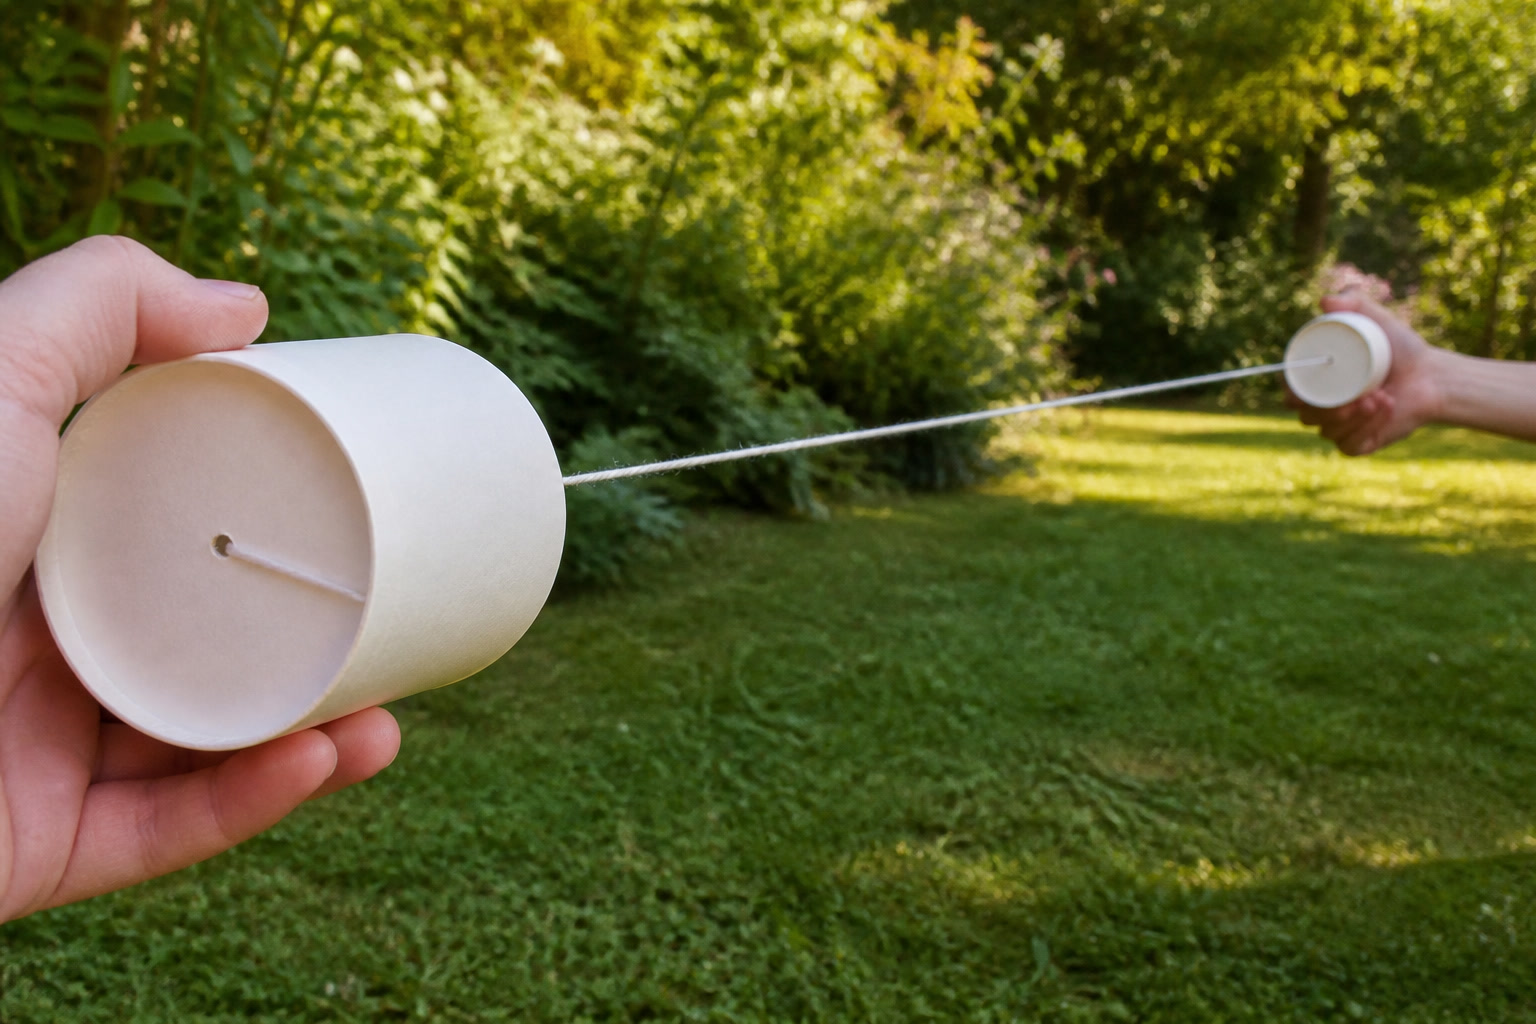
\includegraphics[width=0.58\linewidth]{images/book1/ai/g4-sound-string-telephone.jpg}

{\small O telefone de barbante, armado e esticado: um barbante bem esticado leva o tremor de copinho a copinho muito melhor que o \omterm{def:g2:air-around-us:air}{ar} entre duas pessoas sussurrando.}
\end{omfigure}

\section{O som leva tempo}

\begin{proposition}[Rápido, mas não instantâneo]\label{prop:g4:how-sound-travels:speed}
O \omterm{def:g3:sound-around-us:sound}{som} é um corredor, não um mágico: no \omterm{def:g2:air-around-us:air}{ar} ele percorre cerca de
\qty{340}{m} a cada segundo --- três segundos para mais ou menos um
quilômetro. A \omterm{def:g1:light-and-shadows:source}{luz}, ao contrário, chega tão depressa que, em qualquer
cena que você consiga observar, a viagem dela conta como
instantânea. Essa diferença é a história inteira da tempestade.
\end{proposition}

\begin{method}[A que distância está a tempestade?]\label{met:g4:how-sound-travels:storm}
\begin{enumerate}
  \item Veja o clarão --- comece a contar segundos num ritmo firme:
        mil e um, mil e dois, \dots;
  \item pare no primeiro ronco de trovão;
  \item divida a sua contagem por $3$: esse é mais ou menos o quanto
        a tempestade está distante, em quilômetros.
\end{enumerate}
Seis segundos: cerca de \qty{2}{km}. Contagens cada vez menores entre
um raio e outro querem dizer que a tempestade está se aproximando ---
hora de entrar.
\end{method}

\begin{omfigure}
\begin{tikzpicture}[scale=0.85]
  \draw[thick] (0,0) -- (11,0);
  \draw[very thick, omThm] (1.3,3.4) -- (0.9,2.5) -- (1.25,2.5)
    -- (0.8,1.5) -- (1.15,1.5) -- (0.7,0.4);
  \fill[omExo, opacity=0.3] (0.3,3.4) ellipse (1.5 and 0.45);
  % the listener, counting the silent seconds
  \fill (9.6,1.32) circle (0.18);
  \draw[thick] (9.6,1.14) -- (9.6,0.55);
  \draw[thick] (9.6,1.02) -- (9.33,0.75);
  \draw[thick] (9.6,1.02) -- (9.87,0.75);
  \draw[thick] (9.6,0.55) -- (9.4,0);
  \draw[thick] (9.6,0.55) -- (9.8,0);
  \foreach \r in {0.7, 1.4, 2.1} {
    \draw[omDef, thick] (1.0,0.4) ++(\r,0) arc (0:40:\r);
    \draw[omDef, thick] (1.0,0.4) ++(\r,0) arc (0:-12:\r);
  }
  \node[font=\small, align=center] at (9.15,2.35)
    {``\dots{}cinco, seis''\\--- cerca de \qty{2}{km}};
  \node[right, font=\small, omDef] at (3.6,0.75)
    {o ronco, correndo \qty{340}{m} por segundo};
\end{tikzpicture}

{\small Clarão agora, trovão depois: a \omterm{def:g1:light-and-shadows:source}{luz} chega na hora, o \omterm{def:g3:sound-around-us:sound}{som}
atravessa trotando a \qty{340}{m} por segundo. Os segundos de
silêncio medem a distância.}
\end{omfigure}

\begin{example}[Ecos]\label{ex:g4:how-sound-travels:echo}
Grite na direção de um paredão ou de um prédio isolado lá longe, do
outro lado de um campo: ``ALÔ!'' --- um instante de silêncio ---
``Alô!'' responde a sua própria voz. O \omterm{def:g3:sound-around-us:sound}{som} quica em paredes grandes e
duras, e um \omterm{def:g3:sound-around-us:sound}{som} quicado que volta até você tarde o bastante para ser
ouvido separadamente é um \emph{eco}\index{eco}. Quanto mais distante
a parede, mais longa a viagem de ida e volta da sua voz e mais tarde
o \omterm{ex:g4:how-sound-travels:echo}{eco}. Num cômodo pequeno o quique volta depressa demais para ser
ouvido à parte --- ele só deixa a sua voz mais encorpada.
\end{example}

\begin{remark}[Sonar: o eco posto para trabalhar]\label{rem:g4:how-sound-travels:sonar}
Os navios medem a profundidade do mar gritando para baixo --- um
estalo na água --- e cronometrando o \omterm{ex:g4:how-sound-travels:echo}{eco} vindo do fundo. Água funda,
\omterm{ex:g4:how-sound-travels:echo}{eco} tardio; água rasa, \omterm{ex:g4:how-sound-travels:echo}{eco} rápido. Os golfinhos e os morcegos já
nasceram sabendo o truque: eles estalam e escutam, lendo os \omterm{ex:g4:how-sound-travels:echo}{ecos} para
caçar em água escura e em cavernas de escuridão total. Contando os
segundos do trovão, você já usou o método deles: cronometre o \omterm{def:g3:sound-around-us:sound}{som} e
saiba a distância.
\end{remark}

\section{Exercícios}

\begin{exercise}[$\star$]\label{exo:g4:how-sound-travels:1}
Diga três transportadores de \omterm{def:g3:sound-around-us:sound}{som} deste capítulo e um lugar em que o
\omterm{def:g3:sound-around-us:sound}{som} não consegue viajar de jeito nenhum.
\end{exercise}

\begin{exercise}[$\star$]\label{exo:g4:how-sound-travels:2}
Na experiência do frasco, o martelinho da campainha continua batendo
enquanto o toque morre. O que exatamente foi tirado, e o que isso
prova?
\end{exercise}

\begin{exercise}[$\star$]\label{exo:g4:how-sound-travels:3}
Por que a \omterm{def:g2:moon-in-the-sky:moon}{Lua} é um mundo silencioso? Responda com a proposição do
capítulo.
\end{exercise}

\begin{exercise}[$\star$]\label{exo:g4:how-sound-travels:4}
No telefone de barbante, o que carrega o sussurro? Dê as duas regras
para manter o telefone funcionando.
\end{exercise}

\begin{exercise}[$\star$]\label{exo:g4:how-sound-travels:5}
Que distância o \omterm{def:g3:sound-around-us:sound}{som} percorre pelo \omterm{def:g2:air-around-us:air}{ar} em um segundo, mais ou menos? E
em três segundos?
\end{exercise}

\begin{exercise}[$\star$]\label{exo:g4:how-sound-travels:6}
Você conta nove segundos entre o clarão e o trovão. A que distância
está a tempestade? No raio seguinte, o seu colega conta só três
segundos --- o que mudou, e o que vocês dois devem fazer?
\end{exercise}

\begin{exercise}[$\star$]\label{exo:g4:how-sound-travels:7}
Por que encostar a orelha na mesa deixa você ouvir um arranhão que o
\omterm{def:g2:air-around-us:air}{ar} nunca entregou?
\end{exercise}

\begin{exercise}[$\star$]\label{exo:g4:how-sound-travels:8}
O que é um \omterm{ex:g4:how-sound-travels:echo}{eco}? Por que um paredão maior e mais distante responde
mais tarde que um paredão próximo?
\end{exercise}

\begin{exercise}[$\star$]\label{exo:g4:how-sound-travels:9}
Como o sonar de um navio distingue água funda de água rasa? Quais
dois animais jogam o mesmo jogo, e onde?
\end{exercise}

\begin{exercise}[$\star\star$]\label{exo:g4:how-sound-travels:10}
Os faroestes antigos mostram batedores encostando a orelha no trilho
de aço para perceber um trem ainda distante. Por que o trilho entrega
o trem muito antes do \omterm{def:g2:air-around-us:air}{ar}? Dê as duas vantagens que o trilho oferece
ao \omterm{def:g3:sound-around-us:sound}{som}. (Uma é sobre transportar bem; para a outra, lembre que o
trilho corre em linha reta até o trem, enquanto o \omterm{def:g3:sound-around-us:sound}{som} no \omterm{def:g2:air-around-us:air}{ar} se
espalha em todas as direções, como os anéis num lago, ficando mais
fraco conforme avança.)
\end{exercise}

\begin{exercise}[$\star\star$]\label{exo:g4:how-sound-travels:11}
Parado num pátio grande e vazio, você bate uma palma e ouve o estalo
da sua própria palma voltar da parede distante depois de um segundo
inteiro. O \omterm{def:g3:sound-around-us:sound}{som} correu até a parede e voltou nesse segundo. A que
distância está a parede --- cuidado, pense na viagem de ida e volta!
\end{exercise}
